% !TeX Options = -shell-escape

\documentclass[10pt]{beamer}

\usetheme[progressbar=frametitle, block=fill]{metropolis}
\usepackage{xcolor}
\usepackage{multirow}
\usepackage{pgfpages}
\usepackage{pifont}
\usepackage{hyperref}
\usepackage[utf8]{inputenc}
\usepackage[T1]{fontenc}
\usepackage[english]{babel}
\newcommand{\cmark}{\ding{51}}
\newcommand{\xmark}{\ding{55}}
\setbeamertemplate{note page}{\insertnote}
%\setbeameroption{show notes on second screen=left}
\setbeameroption{hide notes}
\definecolor{amethyst}{rgb}{0.5, 0.4, 1.0}
\definecolor{amethystgrey}{rgb}{0.85, 0.85, 1.0}
\definecolor{amethystdark}{rgb}{0.4, 0.3, 0.9}
\definecolor{orangedark}{rgb}{0.0, 0.9, 0}
%\definecolor{titlebg}{HTML}{4e8074}
%\definecolor{titlebg}{HTML}{3e7985}
\definecolor{titlebg}{HTML}{fbf8ff}
\definecolor{font}{HTML}{23373b}
%\setbeamercolor{title}{fg=amethyst, bg=amethyst}
\setbeamercolor{frametitle}{fg= font, bg=titlebg}
%\setbeamercolor{section title}{black}
%\setbeamercolor{structure}{fg=amethyst, bg=amethyst}
\setbeamercolor{progress bar}{ fg = amethyst, bg= amethystgrey }
%\setbeamercolor{itemize item}{fg=amethyst,bg=white}
\setbeamercolor{alerted text}{fg=amethystdark}
%\setbeamercolor{title separator}{ ... }
%\setbeamercolor{progress bar in head/foot}{ ... }
%\setbeamercolor{progress bar in section page}{ ... }

\newcommand{\code}[1]{\texttt{#1}}

\usepackage{booktabs}
\usepackage[scale=2]{ccicons}

\usepackage{minted}

\usepackage{pgfplots}

\usepackage{xspace}

\title{Coroutines}
\subtitle{All you need to know about the coroutines}
\date{}
\author{Dawid Pilarski}
\institute{dawid.pilarski@tomtom.com \\ blog.panicsoftware.com}


\setminted[c++]
{
framesep=2mm,
baselinestretch=1.2,
fontsize=\footnotesize,
autogobble=true
}

\begin{document}

\maketitle

\begin{frame}{Agenda}
\tableofcontents
\end{frame}

\section{Coroutine theory - what are the coroutines?}

\begin{frame}{What are the coroutines?}
\alert{Coroutines} are \alert{generalization} of the function, that can be:

\begin{itemize}[<+- |alert@+>]
\item created
\item called
\item returned from
\item suspended
\item resumed
\item destroyed
\end{itemize}

\end{frame}

\begin{frame}{Coroutine flowchart}

\begin{columns}
\begin{column}{0.48\linewidth}
  \centering
  Function's flow:
  \vskip 2em
  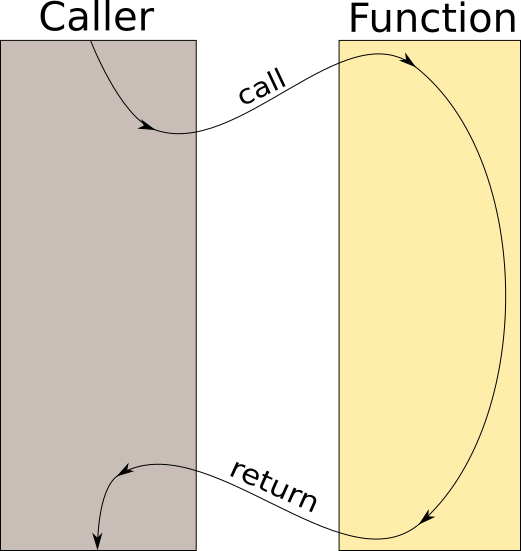
\includegraphics[width=0.8\linewidth]{graphics/function-call.png}
\end{column}

\begin{column}{0.48\linewidth}
  \centering
  Coroutine flow:
  \vskip 2em
  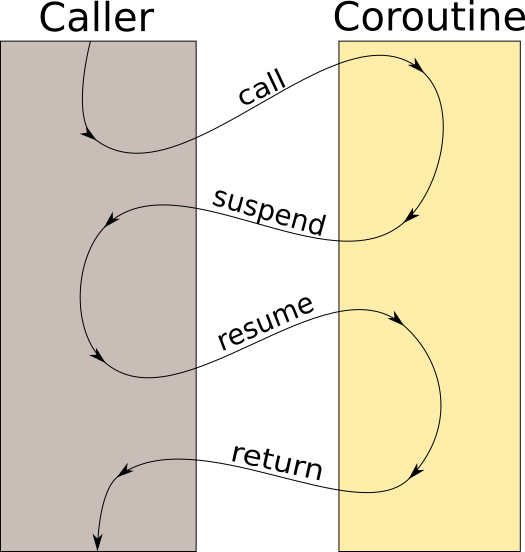
\includegraphics[width=0.8\linewidth]{graphics/coroutine-workflow.png}
\end{column}

\end{columns}

\end{frame}

\begin{frame}{What are coroutines for?}
\centerline{Common use cases for the coroutines are:}
  
      \begin{itemize}
        \item lazy computation of the sequences (generators)
        \item easier asynchronous code
        \item automagical error propagation (more of a hack but still)
      \end{itemize}

  
\end{frame}


\begin{frame}{Possible coroutines implementations}
\begin{columns}[t]
\begin{column}{0.48\linewidth}
  \centering Language based
  \vskip 2em
  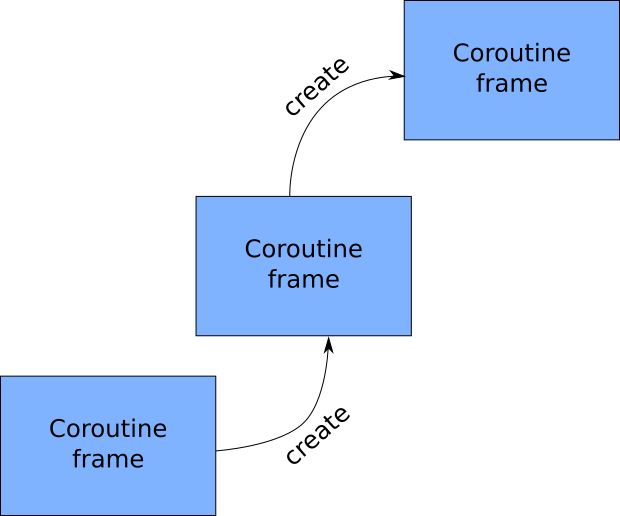
\includegraphics[width=.8\linewidth]{graphics/cppcoro-creation.png}
\end{column}

\begin{column}{0.48\linewidth}
\centering
  Library based
  \vskip 2em
  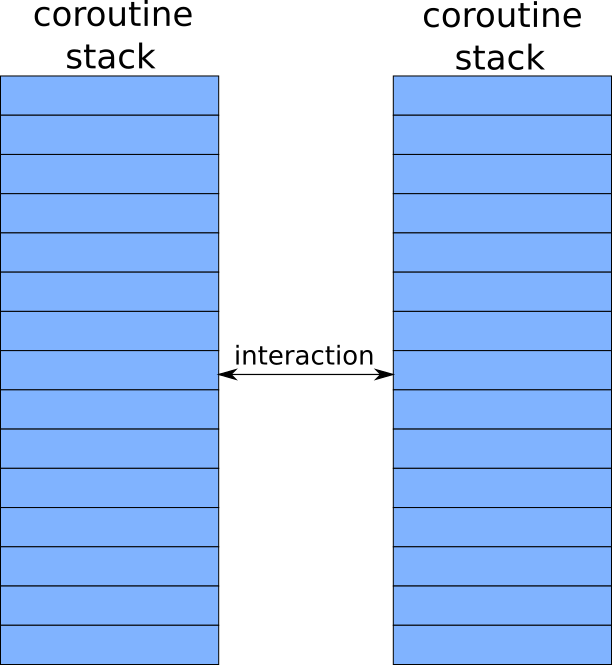
\includegraphics[width=.8\linewidth]{graphics/coroutine-interaction.png}
\end{column}
\end{columns}

\end{frame}

\begin{frame}{Closer look into Boost.Fiber}
  \begin{itemize}[<+- |alert@+>]
  \item Need to allocate the stack for the Fiber/Coroutine
  \item Can be suspended from the top level functions and below
  \item Allocation of the memory in advance
  \item Hard to optimize by compilers
  \end{itemize}
\end{frame}

\begin{frame}{Closer look into built-in coroutines}

  \begin{columns}[t]
  \begin{column}{0.48\linewidth}
  \centerline{Boost.Fiber}
  \vfill
  \begin{itemize}
  \item Need to allocate the stack for the Fiber/Coroutine
  \item Can be suspended from the top level functions and below
  \item Allocation of the memory in advance
  \item Hard to optimize by compilers
  \end{itemize}
  \end{column}
  \begin{column}{0.48\linewidth}
  \centerline{\alert{built-in coroutines}}
  \vfill
  \begin{itemize}[<+- |alert@+>]
  \item Need to allocate the frame for the Coroutine
  \item Can be suspended only from the top level functions
  \item Minimal memory allocation
  \item Easy to optimize by compilers
  \end{itemize}
  \end{column}
  
  \end{columns}
  
\end{frame}

\begin{frame}[fragile]{Coroutine declarations}
  \centering Same as functions

  \vfill
  \begin{center}
  \begin{minipage}{0.7\linewidth}
  \inputminted{c++}{code-examples/intro/declaration.hpp}
  \end{minipage}
  \end{center}
  \vfill

  Whether the function is a coroutine depends on \alert{it's definition}.

\end{frame}

\begin{frame}{3 new keywords}
  \begin{description}
    \item [\code{co\_return}] \hfill \\ Returning (or not) value and finishing the coroutine
    \item [\code{co\_yield}] \hfill \\ Returning intermediate value from the coroutine
    \item [\code{co\_await}] \hfill \\ Awaiting completion of the "task"
  \end{description}
\end{frame}

\section{Practical part I - using cppcoro library}

\begin{frame}{generators - Fibonacci sequence}
  \only{\inputminted[firstline=3, highlightlines={3}]{c++}{code-examples/cppcoro/generator.cpp}}<1>
  \only{\inputminted[firstline=3, highlightlines={4,5}]{c++}{code-examples/cppcoro/generator.cpp}}<2>
  \only{\inputminted[firstline=3, highlightlines={7,18}]{c++}{code-examples/cppcoro/generator.cpp}}<3>
  \only{\inputminted[firstline=3, highlightlines={8}]{c++}{code-examples/cppcoro/generator.cpp}}<4>
  \only{\inputminted[firstline=3, highlightlines={9,10}]{c++}{code-examples/cppcoro/generator.cpp}}<5>
  \only{\inputminted[firstline=3, highlightlines={11,12}]{c++}{code-examples/cppcoro/generator.cpp}}<6>
  \only{\inputminted[firstline=3, highlightlines={13-17}]{c++}{code-examples/cppcoro/generator.cpp}}<7>
\end{frame}

\begin{frame}{generators - excercise}
  % https://edublognss.wordpress.com/2013/04/16/famous-mathematical-sequences-and-series/
  \centering Implement any generator:

  \begin{itemize}
    \item square number series \hskip 2em 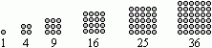
\includegraphics[width=0.3\linewidth]{graphics/square-series.png}
    \item triangular number series \hskip 2em 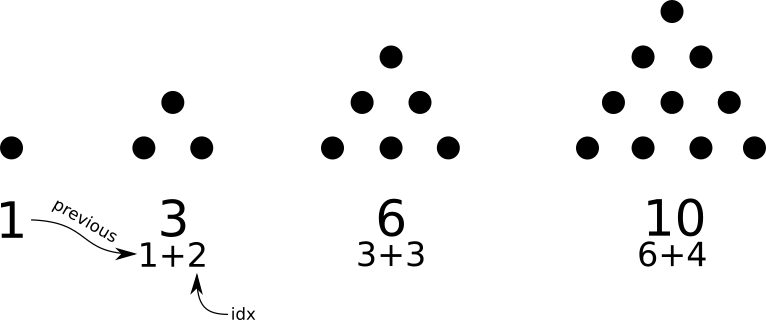
\includegraphics[width=0.3\linewidth]{graphics/triangular-series.png}
  \end{itemize}
\end{frame}

\begin{frame}{tasks and events}
  \only{\inputminted[firstline=48, lastline=63, highlightlines={48, 63}]{c++}{code-examples/cppcoro/events.cpp}}<1>
  \only{\inputminted[firstline=48, lastline=63, highlightlines={49, 56, 57, 63}]{c++}{code-examples/cppcoro/events.cpp}}<2>
  \only{\inputminted[firstline=48, lastline=63, highlightlines={50, 55}]{c++}{code-examples/cppcoro/events.cpp}}<3>
  \only{\inputminted[firstline=48, lastline=63, highlightlines={51}]{c++}{code-examples/cppcoro/events.cpp}}<4>
  \only{\inputminted[firstline=48, lastline=63, highlightlines={52}]{c++}{code-examples/cppcoro/events.cpp}}<5>
  \only{\inputminted[firstline=48, lastline=63, highlightlines={53, 54}]{c++}{code-examples/cppcoro/events.cpp}}<6>
  \only{\inputminted[firstline=48, lastline=63, highlightlines={58, 61}]{c++}{code-examples/cppcoro/events.cpp}}<7>
  \only{\inputminted[firstline=48, lastline=63, highlightlines={59,60}]{c++}{code-examples/cppcoro/events.cpp}}<8>
  \only{\inputminted[firstline=48, lastline=63, highlightlines={62}]{c++}{code-examples/cppcoro/events.cpp} \alert{wtf?}}<9>
\end{frame}

\begin{frame}{other (for now only msvc)}
  \begin{itemize}
    \item mutexes
    \item file I/O operations
    \item networking operations
  \end{itemize}
\end{frame}

\begin{frame}{other (for now only msvc)}
  \only{\inputminted[firstline=4, highlightlines={4}]{c++}{code-examples/cppcoro/io.cpp}}<1>
  \only{\inputminted[firstline=4, highlightlines={6}]{c++}{code-examples/cppcoro/io.cpp}}<2>
  \only{\inputminted[firstline=4, highlightlines={8-11}]{c++}{code-examples/cppcoro/io.cpp}}<3>
  \only{\inputminted[firstline=4, highlightlines={12,17}]{c++}{code-examples/cppcoro/io.cpp}}<4>
  \only{\inputminted[firstline=4, highlightlines={14}]{c++}{code-examples/cppcoro/io.cpp}}<5>
  \only{\inputminted[firstline=4, highlightlines={15-16}]{c++}{code-examples/cppcoro/io.cpp}}<6>
\end{frame}

\section{Theory - promise\_types}

\begin{frame}{promise\_type}
  \begin{itemize}[<+- |alert@+>]
    \item promise\_type is responsible for coroutine's behavior:
    \begin{itemize}
      \item on coroutine's start and stop
      \item on throwing unhandled exception
      \item on returning the value
      \item on yielding the value
      \item partially on waiting for the task's completion
    \end{itemize}
    \item promise\_type is strongly connected with coroutine's returned type
    \begin{itemize}[<+- |alert@+>]
      \item it can be a member of the returned type \code{returned\_type::promise\_type}
      \item it can be defined as \code{std::coroutine\_traits<returned\_type>::promise\_type}
    \end{itemize}
  
  \end{itemize}
\end{frame}

\begin{frame}{coroutine body}
\centerline{Each time we write coroutine, compiler modifies it's body into following form:}
\only{\inputminted[firstline=1, highlightlines={2}]{c++}{code-examples/theory-custom-coroutine/coroutine-body.cpp}}<1>
\only{\inputminted[firstline=1, highlightlines={3}]{c++}{code-examples/theory-custom-coroutine/coroutine-body.cpp}}<2>
\only{\inputminted[firstline=1, highlightlines={4}]{c++}{code-examples/theory-custom-coroutine/coroutine-body.cpp}}<3>
\only{\inputminted[firstline=1, highlightlines={6,8,10}]{c++}{code-examples/theory-custom-coroutine/coroutine-body.cpp}}<4>
\only{\inputminted[firstline=1, highlightlines={7}]{c++}{code-examples/theory-custom-coroutine/coroutine-body.cpp}}<5>
\only{\inputminted[firstline=1, highlightlines={9}]{c++}{code-examples/theory-custom-coroutine/coroutine-body.cpp}}<6>
\only{\inputminted[firstline=1, highlightlines={12,13}]{c++}{code-examples/theory-custom-coroutine/coroutine-body.cpp}}<7>
\only{\inputminted[firstline=1, highlightlines={15}]{c++}{code-examples/theory-custom-coroutine/coroutine-body.cpp}}<8>
\end{frame}

\begin{frame}{promise\_type extensions}
\centerline{We can extend the coroutine body with:}
\begin{itemize}
  \item (mandatory) support for \alert{returning void} or \alert{returning value}
  \item custom memory allocation algorithm (custom \code{operator new})
  \item (optional) support for \alert{yielding intermediate values}
\end{itemize}
\end{frame}

\begin{frame}[fragile]{co\_return - support for returning from coroutine}
\centerline{\alert{\code{co\_return}} is a new keyword}

\begin{columns}[T]
  \begin{column}{0.48\linewidth}
  \vskip 2em
  \centerline{Usage: }
  \vskip 2em
  \begin{onlyenv}<1>

  without expression:
  \begin{minted}{c++}
  co_return 
  \end{minted}

  with void expression:
  \begin{minted}{c++}
  co_return <void expression>
  \end{minted}

  \end{onlyenv}

  \begin{onlyenv}<2>
  with non-void expression:
  \begin{minted}{c++}
  co_return <expression>
  \end{minted}
  \end{onlyenv}

  \end{column}

  \begin{column}{0.48\linewidth}
  \vskip 2em
  \centerline{Translated to: }
  \vskip 2em
  \begin{onlyenv}<1>
   \begin{minted}{c++}
   <expression>;
   promise.return_void();
   goto final_suspend;
   \end{minted}
   \end{onlyenv}
   \begin{onlyenv}<2>
   \begin{minted}{c++}
   promise.return_value(<expression>);
   goto final_suspend;
   \end{minted}
   \end{onlyenv}

  \end{column}
\end{columns}
\end{frame}

\begin{frame}[fragile]{co\_yield - support for returning intemediate values}
\centerline{\alert{\code{co\_yield}} is a new keyword}

\begin{columns}
\begin{column}{0.48\linewidth}
\vskip 2em
Usage:
\vskip 2em

\begin{minted}{c++}
co_yield <non-void expression>
\end{minted}

\end{column}

\begin{column}{0.48\linewidth}
\vskip 2em
Translated to:
\vskip 2em

\begin{minted}{c++}
co_await promise.
         yield_value(<expression>)
\end{minted}

\end{column}
\end{columns}
\end{frame}

\begin{frame}{co\_await shortly}
\begin{description}
  \item[\code{co\_await std::experimental::suspend\_always\{\}}] - \hfill \\ suspends the coroutine
  \item[\code{co\_await std::experimental::suspend\_never\{\}}] - \hfill \\ does nothing
\end{description}

\end{frame}

\begin{frame}{Ok, ok but how do I even resume the coroutine?}
  \centering The low-level interface to the type-erased coroutine is \code{\alert{coroutine\_handle}} object.

  \only{\inputminted[highlightlines={1}]{c++}{code-examples/theory-custom-coroutine/coroutine-handle.h}}<1>
  \only{\inputminted[highlightlines={2,3}]{c++}{code-examples/theory-custom-coroutine/coroutine-handle.h}}<2>
  \only{\inputminted[highlightlines={4}]{c++}{code-examples/theory-custom-coroutine/coroutine-handle.h}}<3>
  \only{\inputminted[highlightlines={6,7}]{c++}{code-examples/theory-custom-coroutine/coroutine-handle.h}}<4>
  \only{\inputminted[highlightlines={9, 10}]{c++}{code-examples/theory-custom-coroutine/coroutine-handle.h}}<5>
  \only{\inputminted[highlightlines={12, 13}]{c++}{code-examples/theory-custom-coroutine/coroutine-handle.h}}<6>
  \only{\inputminted[highlightlines={15}]{c++}{code-examples/theory-custom-coroutine/coroutine-handle.h}}<7>
\end{frame}

\begin{frame}{And how do I get the coroutine\_handle object?}
\centerline{\code{\alert{coroutine\_handles}} are specialized for \code{\alert{promise\_type}}}

  \only{\inputminted[highlightlines={1}]{c++}{code-examples/theory-custom-coroutine/coroutine-handle-promise.h}}<1>
  \only{\inputminted[highlightlines={2}]{c++}{code-examples/theory-custom-coroutine/coroutine-handle-promise.h}}<2>
  \only{\inputminted[highlightlines={4}]{c++}{code-examples/theory-custom-coroutine/coroutine-handle-promise.h}}<3>
  \only{\inputminted[highlightlines={5, 10}]{c++}{code-examples/theory-custom-coroutine/coroutine-handle-promise.h}}<4>
  \only{\inputminted[highlightlines={6, 8}]{c++}{code-examples/theory-custom-coroutine/coroutine-handle-promise.h}}<5>


\end{frame}

\section{Promise\_type excercise}

\begin{frame}{promise\_type excercise - lazy}
\centerline{type for lazy initialization}
\vfill
requirements:
\begin{itemize}
  \item synchronous (no support for multithreading + no support for co\_await).
  \item no sharing of the value (no copy, only move constructor).
  \item interface simillar to the std::optional.
\end{itemize}
\end{frame}

\begin{frame}{promise\_type excercise - generator}
  \centerline{type for generating sequences}
  \vfill
  requirements:
  \begin{itemize}
    \item synchronous (no support for multithreading + no support for co\_await).
    \item next method should return the value and resume the coroutine.
    \item interface simillar to the std::optional
  \end{itemize}
\end{frame}

\section{Asynchronous coroutines}

\begin{frame}{co\_await}
\centerline{\alert{co\_await} is a new keyword}

\begin{itemize}
  \item represents awaiting for operations' completion
  \item it's argument is (usually) called awaitable
  \item it's result is usually called awaiter
\end{itemize}
\end{frame}

\begin{frame}{co\_await translation}
\centerline{If compiler meets the co\_await it gets translated into following code:}

\only{\inputminted[highlightlines={3, 7}]{c++}{code-examples/theory-custom-coroutine/co-await-transformation.cpp}}<1>
\only{\inputminted[highlightlines={9, 12}]{c++}{code-examples/theory-custom-coroutine/co-await-transformation.cpp}}<2>
\only{\inputminted[highlightlines={4}]{c++}{code-examples/theory-custom-coroutine/co-await-transformation.cpp}}<3>
\only{\inputminted[highlightlines={6, 2}]{c++}{code-examples/theory-custom-coroutine/co-await-transformation.cpp}}<4>
\only{\inputminted[highlightlines={12}]{c++}{code-examples/theory-custom-coroutine/co-await-transformation.cpp}}<5>
\only{\inputminted[highlightlines={10, 11}]{c++}{code-examples/theory-custom-coroutine/co-await-transformation.cpp}}<6>
\end{frame}

\begin{frame}[fragile]{Await suspend}
% nothing yet said about the coroutine_handle
\centerline{await suspend is of the following form:}
\begin{minted}[autogobble=false]{c++}
               promise.await_suspend(this_coroutine_handle);
\end{minted}

\centerline{\code{await\_suspend} might return:}
\vskip 1em
\hrule

\begin{columns}
\begin{column}{0.35\linewidth}
\begin{itemize}[<+- |alert@+>]
\item \code{void}
\item \code{bool}
\item \code{coroutine\_handle}
\end{itemize}
\end{column}

\begin{column}{0.66\linewidth}
\begin{onlyenv}<1>
\inputminted[firstline=1, lastline=9, linenos=false]{c++}{code-examples/theory-custom-coroutine/co-await-transformation-suspend.cpp}
\end{onlyenv}
\begin{onlyenv}<2>
\inputminted[firstline=10, lastline=20, linenos=false]{c++}{code-examples/theory-custom-coroutine/co-await-transformation-suspend.cpp}
\end{onlyenv}
\begin{onlyenv}<3>
\inputminted[firstline=21, linenos=false]{c++}{code-examples/theory-custom-coroutine/co-await-transformation-suspend.cpp}
\end{onlyenv}
\end{column}
\end{columns}

\end{frame}

\begin{frame}[fragile]{Awaitable and Awaiter}
\alert{Awaitable} is an object, which is an operand of the co\_await operator

\alert{co\_await <expression>} expression will be processed in following manner

\vskip 2em

\begin{columns}
\begin{column}{0.4\linewidth}
\begin{itemize}[<+- |alert@+>]
  \item await\_transform
  \item acquiring awaiter
  \begin{itemize}[<+- |alert@+>]
  \item co\_await operator
  \item global co\_await operator
  \item awaitable to awaiter
  \end{itemize}
\end{itemize}
\end{column}

\begin{column}{0.56\linewidth}
\footnotesize
\begin{onlyenv}<1>
  is performed only if promise has await\_transform function declared
  \vskip 2em

  \begin{minted}{c++}
  co_await promise.await_transform(<expr>);
  \end{minted}
\end{onlyenv}

\begin{onlyenv}<3>
  is performed only if awaitable has co\_await operator

  \begin{minted}{c++}
  auto&& awaiter = 
         <awaitable>.operator co_await();
  \end{minted}
\end{onlyenv}

\begin{onlyenv}<4>
  is performed only if awaitable there is matching global co\_await operator

  \begin{minted}{c++}
  auto&& awaiter = 
         operator co_await(<awaitable>);
  \end{minted}
\end{onlyenv}

\begin{onlyenv}<5>
  \begin{minted}{c++}
  auto&& awaiter = <awaitable>;
  \end{minted}
\end{onlyenv}

\end{column}
\end{columns}
\end{frame}

\section{Asynchronous coroutines - excercises}

\begin{frame}{task}
  \centerline{type for asynchronous operations}
  \vfill
  requirements:
  \begin{itemize}
    \item single-threaded
    \item asynchronous (support for the co\_await)
    \item coroutine after finishing must resume the co\_awaiting coroutine
    \item some kind of the executor needed to start the coroutines (GitHub)
  \end{itemize}
\end{frame}

\begin{frame}{event}
  \centerline{type for communication of the tasks}
  \vfill
  requirements:
  \begin{itemize}
  \item stores information whether the event is set.
  \item stores the continuation object.
  \item launches the continuation on setting up the event.
  \end{itemize}
\end{frame}

\begin{frame}{Thank you!}
\centerline{Questions?}
\vfill

\begin{columns}[t]
\footnotesize
\begin{column}{0.48\linewidth}
\centerline{recommended lecture:}
\vskip 0.5em
\hrule
\begin{itemize}
  \item \href{https://lewissbaker.github.io/}{\alert{Lewiss Baker blog}}
  \item \href{https://blog.panicsoftware.com/}{\alert{My blog}}
  \item \href{https://programistamag.pl/}{\alert{"programista" magazine}}
  \item \href{eel.is/c++draft/}{\alert{current C++ standard draft}}
  \item {coroutine channel on cpplang slack}
\end{itemize}
\end{column}

\begin{column}{0.48\linewidth}
\centerline{recommended videos:}
\vskip 0.5em
\hrule
\begin{itemize}
  \item \href{https://www.youtube.com/watch?v=8C8NnE1Dg4A}{\alert{Gor Nishanov \\ "C++ Coroutines: Under the covers"}}
  \item \href{https://www.youtube.com/watch?v=mlP1MKP8d_Q}{\alert{Toby Allsopp \\ "Coroutines: what can't they do"}}
  \item \href{https://www.youtube.com/watch?v=ZTqHjjm86Bw}{\alert{James McNellis \\ "Introduction to C++ Coroutines"}}
\end{itemize}
\end{column}
\end{columns}

\end{frame}

\end{document}